\documentclass[12pt]{article}

\renewcommand{\baselinestretch}{2.0}
\usepackage{indentfirst}
\usepackage[a4paper, left=25mm, top=25mm, bottom=25mm, right=25mm]{geometry}
\usepackage{setspace}
\usepackage{tikz-er2}
\usetikzlibrary{positioning}
\usepackage{graphicx}
\graphicspath{{../Figures/}}
\usepackage{multirow}

\tikzstyle{every entity} = []
\tikzstyle{every weak entity} = []
\tikzstyle{every attribute} = [node distance=1cm]
\tikzstyle{every relationship} = []
\tikzstyle{every isa} = []

\title{CMPSC 431W Project Proposal\\Team: Big Leg Carry}
\author{
	Sui, Haojun\\
	\texttt{hzs5220@psu.edu}
	\and
	Deng, Yuanpei\\
	\texttt{dengyuanpei@gmail.com}
	\and
	Zhang, Chenyu\\
	\texttt{dianachenyuzhang@gmail.com}
	\and
	Wang, Hao\\
	\texttt{haowang5128@gmail.com}
	\and
	Chen, Shiqing\\
	\texttt{u0vv0u@gmail.com}
}
\date{\today}


\begin{document}
\maketitle
\thispagestyle{empty}
\newpage
\tableofcontents
\pagenumbering{roman}
\setcounter{page}{1}
\newpage
\listoffigures
\newpage
\listoftables
\newpage

\pagenumbering{gobble}
\pagenumbering{arabic}

\section{Introduction}
HelloWorld is a startup company that wants to pursue the opportunities of online business. We, team Big Leg Carry, have designed a database application for online Car shopping for HelloWorld. Users may log into our system by using registered user account or seller account. Registered users may easily search the kind of cars they want from search page, or they can fill out our quick survey to see what kind of cars suit their need. Users may compare different cars at the same time, if they are interested in multiple cars and have a hard time to choose the best one. Registered users may purchase a vehicle or place a bid on the vehicle. Once the transaction is confirmed, users can either choose to have vehicle delivered to them, or pick the vehicle themselves. Upon receiving the cars, users must finish the rest of the payment. Sellers can easily list the vehicles they want to sell from sellers' webpage. Both registered users and sellers can make rating on each other. We want such feature to maintain our friendly ecosystem. In order to fulfill these features, we define the following requirements.

\newpage

\section{Requirement Analysis}
\subsection{Sale Items}
The items that we are offering for sale are automobiles. Items listed on our websites are stored in a database management system as an entity. Each item will have a primary key named the item\_id which is unique to every item. As to offer better details to item listings as well as the sake of searching features. Several attributes will be present for the item entity. Some attribute will be visible to the customers as item specifics, and some will be only visible to those who have access to our database as listing specifics. The item specifics include Vehicle Make, Vehicle Condition, Vehicle Model, VIN (Vehicle Identification Number), Year, Mileage, Vehicle Title, Vehicle Type, Body Type, Options, Safety Features, Power Options, Sub Model, Fuel Type, Exterior Color, Interior Color, Drivetrain, For Sale By, Number of Cylinders, Engine Description, Transmission, Trim, and Warranty. On the other hand, the listing specifics indicators include Listing Status, Listing Type, Listing Duration, and Listing Start Time.\par
As most of these item specifics are very straightforward, some still need further clarification. Vehicle Title refers to the current status of a vehicle, and has two types: clean title and clear title. A clean title is usually used to refer to any car that passes inspection without having any serious physical issues. A clear title is usually used to describe a financial lien that has been placed on a car. For Sale By refers to the type of the seller, which can be either dealer or individual seller. For listing specifics, listing status refers to the status of the listings, and can be active, ended, unsold, sold, and removed. Listing Type can be either auction or buy-it-now. Listing Duration is the time period when the listing is active.

\subsection{Categories}
``Shop by Categories" is a necessary way to browse items as customers may not know what to search. The items available at HelloWorld are categorized using a predefined classification tree. Customers will first choose the body type of the vehicle. So the root of the tree will be labeled as ``All Body Type", which we have the nodes of the root as SUV, Pickup Truck, Convertible, Sedan, Crossover, Coupe, Luxury Car, Wagons/Hatchback, Green Cars/Hybrids, Sports Cars, and Minivans/Vans. On the lower levels of the first tree, from top to the bottom, we have: Make, Year, Model, Sub Model, and Trim. \par
An item can be specified by a path through this classification tree. For example, we may
categorize an item as:
\begin{enumerate}
\item SUV $>$ Audi $>$ 2016 $>$ Q7 $>$ Q7 eTron $>$ Base\par
\item All Body Type $>$ Fiat $>$ 2011 $>$ 500 $>$ 500 Abarth\par
\end{enumerate}
\par The depth of the tree varies but is no more than ten levels deep.

\subsection{Suppliers}
In our case, supplier is the car seller. The attributes of supplier (dealer) are dealer name, address, phone number, type, account number, and rating. The type attribute classifies supplier as car dealer and individual seller. The dname here is used as the primary ID and required to be unique. Phone numbers, rating, type, etc are attributes connected to each dealer. The rating is a weighted score calculated by buyer's (register user) rating on aspects like accuracy, price, choice, service, and feedback. Dealer will have an inventory. The relation is called owns and the entity is cars. The cars table is discussed in detail in the above sale items section. The dealer also has a relation named locates and the entity is address. The address we used here is zip code. Address is an important attribute in car shopping. People would prefer a dealer near their location so that they can go to store for a test drive and get car service there after the purchase. The address would be used in the search to decrease the scope. The reason we choose make ``address'' as an entity instead of an attribute is that we can use the similar schema for registered users. Figure \ref{ERSupp} shows the ER diagram for Suppliers.
\begin{figure}[!h]
\caption{ER diagram for Suppliers.\label{ERSupp}}
\begin{center}
\begin{tikzpicture}[node distance=1.5cm, every edge/.style={link}]
	\node[entity] (dealer) {Dealers};
	\node[attribute] (dealername) [left=of dealer] {\key{dname}} edge (dealer);
	\node[attribute] (phone) [above=of dealer] {phone} edge (dealer);
	\node[attribute] (account) [below left=of dealer] {account} edge (dealer);
	\node[attribute] (rating) [right=of dealer] {rating} edge (dealer);
	
	\node[relationship] (owns) [below=of dealer] {Owns} edge (dealer);

	\node[entity] (car) [below=of owns] {Cars} edge (owns);

	\node[relationship] (locates) [below right=of dealer] {Locates} edge (dealer);
	
	\node[entity] (address) [below right=of locates] {Address} edge (locates);
\end{tikzpicture}
\end{center}
\end{figure}

\subsection{Registered Users}
The registered users are the buyers who can buy or bid on an item (car). Buyer must be registered, and identified by a user name and authenticated with a password. When registering, the user would be asked the following information in order to register successfully. These information includes: email address, name, address, phone number and credit card info like type of card, card number, cvv and expiration date. Figure \ref{registered_users} shows how the interface of registering page looks like for Madison, Inc. (In real design the credit card information will be added.)
\begin{figure}[!h]
\caption{Interface of Registering Page for Madison, Inc.} \label{registered_users}
\begin{center}
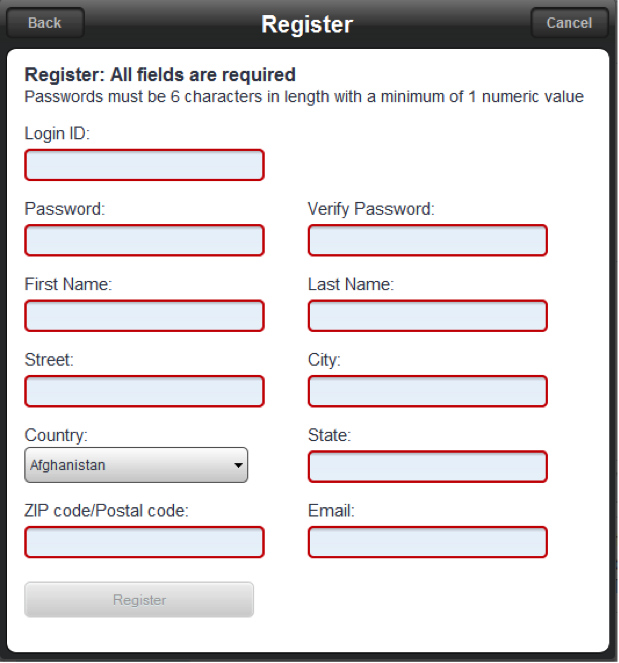
\includegraphics[width=13cm]{registered_users}
\end{center}
\end{figure}
\par In addition, after registering a user can complete his or her whole profile by adding other information like age, gender and annual income. These attributes can be NULL if the user chooses not to fill.\par
Register user also has a rating attribute. A new user has a rating of 0 to start with and recalculates his or her rating score after each successful business. Figure \ref{ERUser} shows the ER diagram for registered users.
\begin{figure}[!h]
\caption{ER diagram for Registered Users.\label{ERUser}}
\begin{center}
\scalebox{.70}{
\begin{tikzpicture}[node distance=1.5cm, every edge/.style={link}]
	\node[entity] (user) {Users};
	\node[attribute] (age) [left=of user] {Age} edge (user);
	\node[attribute] (username) [above left=of age] {\key{username}} edge (user);
	\node[attribute] (gender) [above left=of user] {Gender} edge (user);
	\node[attribute] (password) [above right=of gender] {Password} edge (user);
	\node[attribute] (income) [above right=of password] {Income} edge (user);
	\node[attribute] (email) [above right=of user] {Email} edge (user);
	\node[attribute] (rating) [above=of gender] {Rating} edge (user);
	
	\node[ident relationship] (has) [below left=of user] {Has} edge (user);
	
	\node[weak entity] (phone) [left=of has] {Phones} edge [total] (has);
	\node[attribute] (pnumber) [below=of phone] {\discriminator{Phone number}} edge (phone);
	
	\node[relationship] (pay) [below=of user] {Pays by} edge (user);
	
	\node[entity] (credit) [below=of pay] {Credit Cards} edge [total] (pay);
	\node[attribute] (exp) [left=of credit] {Expiration Date} edge (credit);
	\node[attribute] (type) [below=of credit] {Type} edge (credit);
	\node[attribute] (cnumber) [right=of credit] {\key{Card Number}} edge (credit);
	
	\node[relationship] (live) [right=of user] {Lives in} edge (user);
	
	\node[entity] (address) [right=of live] {Addresses} edge [total] (live);
	\node[attribute] (state) [above=of address] {State} edge (address);
	\node[attribute] (city) [above right=of address] {City} edge (address);
	\node[attribute] (street) [right=of address] {\key{Street}} edge (address);
	\node[attribute] (zip) [below right=of address] {Zip} edge (address);
	
	\node[relationship] (use) [below right=of user] {Uses} edge (user);
	
	\node[entity] (name) [below right=of use] {Name} edge (use);
	\node[attribute] (last) [right=of name] {Last} edge (name);
	\node[attribute] (first) [below right=of name] {First} edge (name);
\end{tikzpicture}
}
\end{center}
\end{figure}

\subsection{Rating}
Each supplier and register user has a rating score to reflect their past business behaviors with other users. For suppliers who sell cars on the website, the rating is an importing factor to help customers, the register users, to compare service quality and make purchase decision. For register users who are customers or potential customers, the rating reflects a general feedback from the car sellers and their punctuality of payment. Mostly, the rating of supplier is more important compared to that of user but we would have ratings for both supplier and register user.\par
Each successful business would allow one rating. Supplier and register user would rate each other on the scale of 1-10. Suppliers would be rated on the aspects of accuracy, price, choice, service, and feedback.\par
\begin{enumerate}
\item Accuracy: If the information online the same as the real condition of the car.
\item Price: Price is probably one of the most important factors for used car shopping. Is the price provided by the dealer competitive compared to others'?
\item Choice: Does the dealer provide a lot of car choices?
\item Service: Is the dealer professional, nice, and informative? Does the dealer respond your call and emails in a timely manner? Does the dealer call you way too frequently and become bothering?
\item Feedback: The customer can add more feedback months or even years after the purchase. Is the car still working well after a year? For register user/buyer, the rating from supplier would be simpler. If the register users are new and did not purchase on the website before, they would start with a score of 0. It would be the case for most of the register users, especially at the beginning of website operation. The register user would be rated on feedback and payment punctuality.
\item Feedback: Is the register user a good and reasonable customer?
\item Payment: Does the customer pay the rest of money on time? Does customer finish the loan at the end as planned?
\end{enumerate}

\subsection{Browsing}
Browsing is one of the most important feature of a website, especially for a car selling website. It has great impact on user experience for the website, a good browsing feature can give user easy access to the target items, however, a bad browsing feature will prevent user from accessing the target items and sometimes even browse the wrong items.\par
\textbf{\underline{How it works}}\par
According to the input, using SQL to select proper table or a specific record. Users are able to browse the items by traversing the category tree. At each point, they are given a summary of all the items that appear in that category.\par
\textbf{\underline{Design}}\par
A good browning feature should have the following attributes:\par
\begin{enumerate}
\item Easy to use (good design)
\item Accurate (well built database and proper SQL instructions)
\item Quick response (well built database and proper SQL instructions)
\end{enumerate}
\par Browsing is usually done by a browsing bar. There are two types of browsing bar in our website: horizontal bar and vertical bar. Horizontal bar is on the top of the page and vertical bar (box) is on the right of the page.\par
Horizontal bar consists of 2 buttons and 3 drop-down menus (See in Figure \ref{horBar}):
\begin{figure}[!h]
\caption{Horizontal Bar Design.} \label{horBar}
\begin{center}
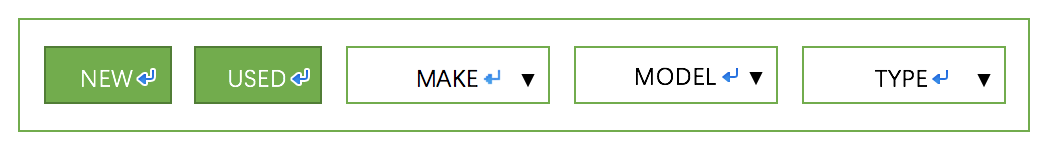
\includegraphics[width=\textwidth]{horizontal_bar}
\end{center}
\end{figure}
\par On the main page, browsing bar is placed horizontally on top of the page which is a striking position. By doing this, it provides easy access for users to browse our inventory right after they enter the website.\par
\underline{New Car button and Used Car button:} User can select New car, used car, or both to browse our inventory. User can combine buttons with drop-down menus to filter out undesired results. Results will be displayed after button selection.\par
\underline{Drop-down menus:} For users who have a target car in mind. First, select make of the car and then select model will take them to the result selected from our database according to the given input. Or users can browse the car by type (sedan, coupe, SUV, other), and jump to the result page with cars of that type.\par
All inventory pages have a vertical browse bar with all the attributes according to previous input (new/used/type...) Figure \ref{verBar} shows the design of the vertical bar.
\begin{figure}[!h]
\caption{Vertical Bar Design.} \label{verBar}
\begin{center}
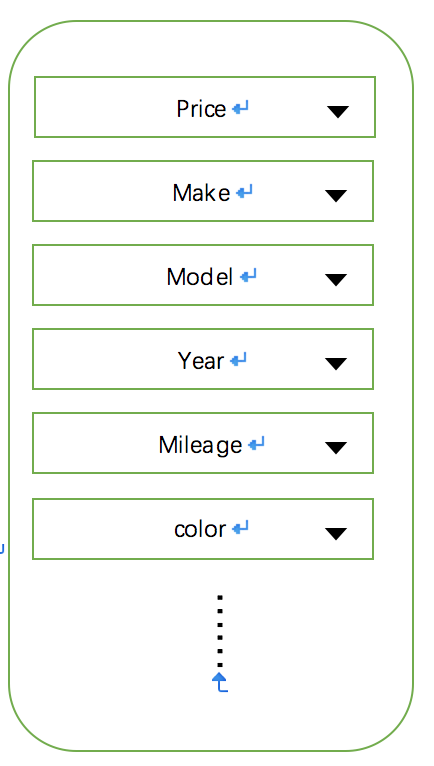
\includegraphics[width=9cm]{vertical_bar}
\end{center}
\end{figure}
\par The reason that it is on vertical and on the right is that user are not disturbed by drop-down menus and focus more one the content.\par
Every change of the drop-down menu will immediately execute a SQL instruction and bring the result to the page.

\subsection{Searching}
Users are able to search the items by entering some keywords or conditions. As a search result, a list of items that satisfy the search criteria is returned to the users.
Searching is another function to get quick access to the target item besides browsing. If a user has a specific car in mind, by using our search bar, he can filter out the non-matching records and gets the desired results directly from our database.\par
\textbf{\underline{How it works}}\par
User types a keyword in the search bar and hit enter to search. Website breaks the keyword into several words. The website will search the first word in all the related tables in our database, then search the next word in the result from last word searching.\par
\textbf{\underline{Simplified Example}}\par
Assume user search for Audi A5, we breaks the search words into keywords `Audi', `A5'. We first search for Audi. Figure \ref{search_example_audi} shows the results to users.
\begin{figure}[!h]
\caption{Search for Audi.} \label{search_example_audi}
\begin{center}
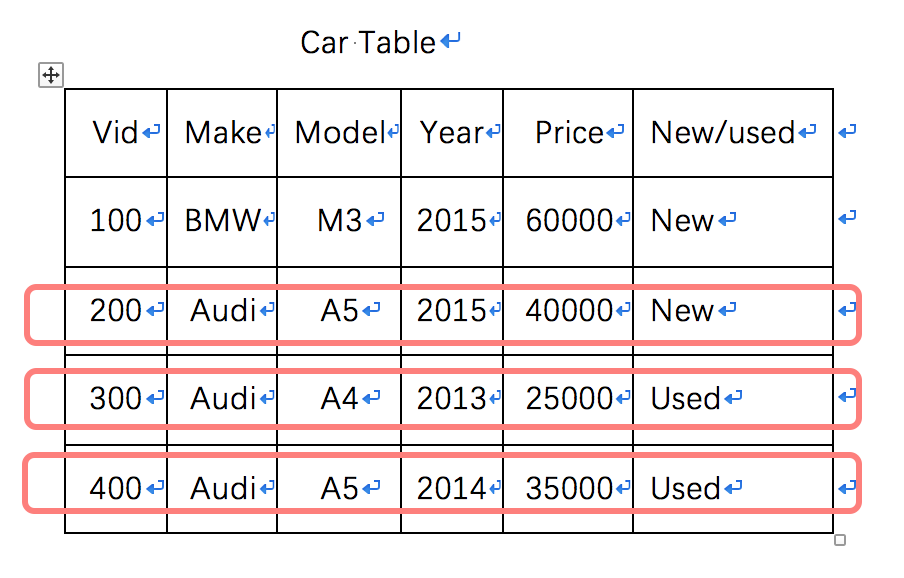
\includegraphics[width=9cm]{search_example_audi}
\end{center}
\end{figure}
\par We then search for A5. Figure \ref{search_example_a5} shows the results to users.
\begin{figure}[!h]
\caption{Search for A5.} \label{search_example_a5}
\begin{center}
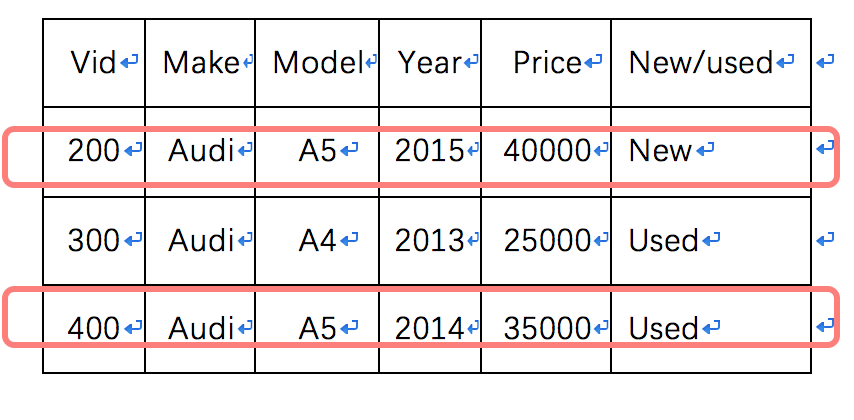
\includegraphics[width=9cm]{search_example_a5}
\end{center}
\end{figure}
\par \textbf{\underline{Design}}
\par Figure \ref{search_bar} shows the design of the search bar.
\begin{figure}[!h]
\caption{Search Bar Design.} \label{search_bar}
\begin{center}
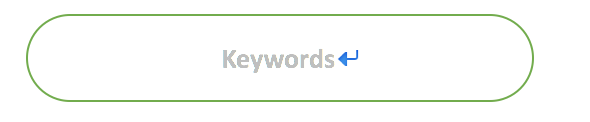
\includegraphics[width=9cm]{search_bar}
\end{center}
\end{figure}
\par It will be on every page, together with browsing bar so that user can perform a search no matter what page they are on.

\subsection{Sale}
When a buyer decide to purchase an item (car), the website will charge the buyer?s credit card the amount of the price of the item and the delivery fee.  The website will hold it until the buyer confirmed that the car is delivered. Then the website will transfer the money to the seller. Then this transaction is closed.

\subsection{Bidding}
At HelloWorld, bidding is pretty easy and fair. When seller lists a vehicle on our website, he can choose auction as the listing type. Then he will set a starting price for the auction, a duration, and a reserve price as an optional feature. The starting price has to be greater than 0.99, and lower than the item's buy-it-now price if it has one. The duration can be 3 days, 5 days, and 7 days max. The reserve price which is invisible to buyers is the price threshold where buyers have to bid higher price than the reserve price in order to win the item. If no bid achieves the reserve price at the time when the listing ends, then the item isn't sold. Seller can't change an auction type listing to fixed price listing, but he may end an auction earlier than the projected end time. Seller can change a fixed price listing to an auction type at any time before the end of the listing period, and then the auction duration will be added to the listing upon a successful change from fixed price to auction. To maintain the fairness of the auction, bidders are anonymous to sellers, only the highest bid is visible to the seller. \par
On the buyer side, one can bid on any item at any time, and the number of bids is unlimited. There are two types of bids, one is a one-click-bid, and the other is a max-bid. A one-click-bid is the bid which is one bid increment higher than the current bidding price. The bid increment is determined by the range of current bidding price. Table \ref{pricebid} shows the current bid increment.
\begin{table}[!h]
\caption{Current Price Bid Increment}\label{pricebid}
\begin{center}
\begin{tabular}{|l|c|}
\hline
Price Range(\$) & Bid Increment(\$)\\ \hline
Up to 99.99 & 5\\ \hline
100 to 999.99 & 25\\ \hline
1000 to 4999.99 & 50\\ \hline
5000 to 9999.99 & 100\\ \hline
10000 to 49999.99 & 200\\ \hline
50000 or more & 500\\ \hline
\end{tabular}
\end{center}
\end{table}
\par The max bid is the maximum price a buyer is willing to pay for the item. The max bid is required to be at least one bid increment higher than the current price. When a buyer placed a max bid on an item, the current bid will raise only one bid increment. Buyer can raise the max bid any time during the auction. All the one-click-bids are visible to all the buyers, but max bids are only visible to the buyer who placed it. Buyer can retract his bid any time during the auction, and only if the bid is the highest bid at the moment, but leaving a record of retraction. After retraction, the highest bid placed by other buyer will be the current bid. When buyer A places a bid higher than the current bidding price, buyer B with that bid will be outbid, which means the buyer B will have to bid higher in order to win the item. If buyer B has a max bid, then the bid from buyer A may not be high enough to compete, then buyer A will be automatically outbid with a bid increment at the current bidding range. Buyer A will then place higher bids until the highest bid is lower than his max bid. The highest bid at the end of auction is called a winning bid, the buyer who placed the bid will be the winner of the auction. However, if the highest bid isn't higher than the reserve price, then the buyer isn't winning.

\subsection{Order and Sale Reports}
Every week, a report would be generated to summarize all the sale and website traffic information happened in the past week. Table \ref{report_element} contains the order and report elements.
\begin{table}[!h]
\caption{Order and Report Elements}\label{report_element}
\begin{center}
\begin{tabular}{|c|c|}
\hline
Section & Elements\\ \hline
\multirow{3}{*}{Sale} & Total number of business transaction\\
& Total number of car sold\\
& Total amount of sale figure(money)\\ \hline
\multirow{3}{*}{Traffic} & Total number of visits\\
& Pages viewed per visit\\
& Average time spent per visit\\ \hline
\multirow{3}{*}{Figure and Comparison} & 	Percentage of increment/decrement compared to last week\\
& The category with the largest change\\
& Visual representation of graphs and figures \\ \hline
\end{tabular}
\end{center}
\end{table}

\subsection{Delivery}
After the buyer bought the vehicle from our website, two options of delivery will be offered. Buyer can drive to the dealer to pick up the vehicle, or he can use our insured and convenient delivery services. If the buyer chooses to pick up the vehicle, he will complete the paper work and pay the vehicle price in full excluding the deposit when he arrives in the dealer?s. Buyer may have a test drive with the car, but he can't retract the purchasing agreement consented on our website. In the worst case, if the buyer persists that he can't purchase the car, the buyer will be charged a penalty no more than 5\% of the final price.\par
The vehicle delivery services we provide on our website are offered by two partner: the Nittany Auto Delivery, and Tennis Auto Delivery. Both our partners have strongly skilled drivers with sales skills, and their offices are located all over the country. If a buyer choose to get the vehicle via one of the delivery partners, he can expect the vehicle at his door after 3-7 business days upon clear payments. The charges of the delivery will be determined on the distance between the two destination and the type of the vehicle. The optional insurance on the auto delivery will be offered at buyer's expense. At the time when the car is delivered to the buyer, buyer will complete the payments as well as paperwork with the trusted driver from our partners. Figure \ref{delivery} shows shipping quotes from ebay.com.
\begin{figure}[!h]
\caption{Shipping quotes from ebay.com.} \label{delivery}
\begin{center}
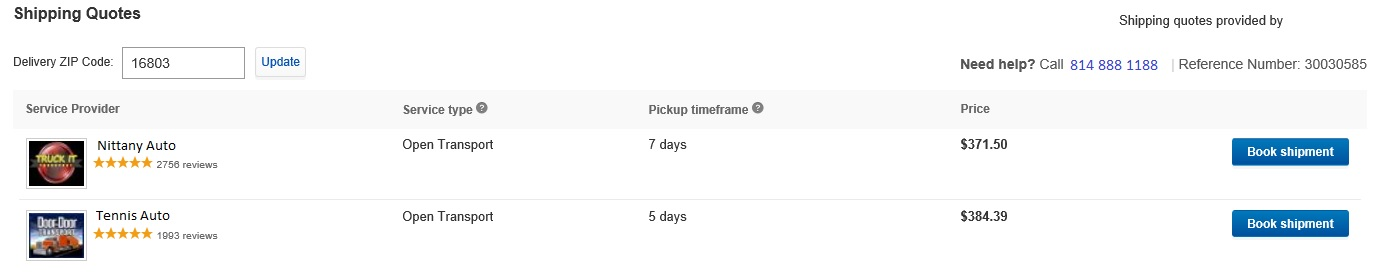
\includegraphics[width=13cm]{delivery}
\end{center}
\end{figure}

\subsection{Smart Car Finder}
For user who do not have a target car in mind or do not have knowledge about cars, car find will give them recommendations according to their needs.\par
\textbf{\underline{How it works}}\par
User will take a short multiple choice survey. Car finder transfer the user-answers and transfer to proper keywords to browse the database and filter out the undesired results. After finishing the survey, what final results will show on the page.\par
\textbf{\underline{Design}}\par
The questions in the survey are written in descriptive words instead of professional terms of a car. For example, survey will have expression like ``big car'', ``large cargo space'' instead of ``SUV'' since user may not know what is SUV. The survey will ask user in an easy way and get the following information from user: Price range, car type, mpg range, year of manufacture or other feature like backup cam, FWD/AWD, etc. Survey can be accessed by clicking ``help me to find a car'' button. 

\subsection{Item Comparison}
Since this is car purchasing, user probably need compare several cars to determine which one to buy. So compare function is very important for this project. After the user searching for what kinds of car he wants to buy, there will be a list of cars that satisfied his searching key word. Figure \ref{car_comparison} shows how Cars.com implements the same kind of feature.
\begin{figure}[!h]
\caption{Car Comparison from Cars.com.} \label{car_comparison}
\begin{center}
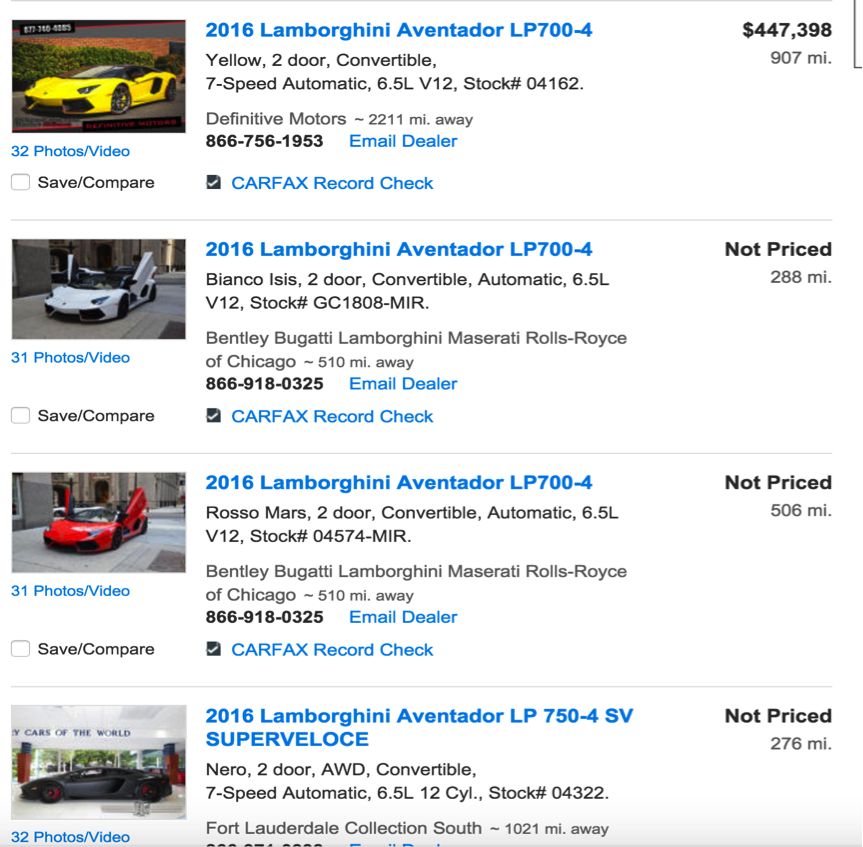
\includegraphics[width=13cm]{car_comparison}
\end{center}
\end{figure}
\par Then user can mark several cars as compare. On the top of website there will be a button ``compare''. By clicking this button the website will generated a table shows the data of the marked cars? entities.

\newpage

\section{Conceptual Design}
Figure \ref{ERCom} shows the complete ER diagram design of our database application.
\begin{figure}[!h]
\caption{Complete ER diagram Design.\label{ERCom}}
\begin{center}
\scalebox{.55}{
\begin{tikzpicture}[node distance=1.5cm, every edge/.style={link}]
	\node[entity] (user) {Users};
	\node[attribute] (age) [left=of user] {Age} edge (user);
	\node[attribute] (username) [above left=of age] {\key{username}} edge (user);
	\node[attribute] (gender) [above left=of user] {Gender} edge (user);
	\node[attribute] (password) [above right=of gender] {Password} edge (user);
	\node[attribute] (income) [above right=of password] {Income} edge (user);
	\node[attribute] (email) [above right=of user] {Email} edge (user);
	\node[attribute] (rating) [above=of gender] {Rating} edge (user);
	
	\node[ident relationship] (has) [below left=of user] {Has} edge (user);
	
	\node[weak entity] (phone) [left=of has] {Phones} edge [total] (has);
	\node[attribute] (pnumber) [below=of phone] {\discriminator{Phone number}} edge (phone);
	
	\node[relationship] (pay) [below=of user] {Pays by} edge (user);
	
	\node[entity] (credit) [below=of pay] {Credit Cards} edge [total] (pay);
	\node[attribute] (exp) [below right=of credit] {Expiration Date} edge (credit);
	\node[attribute] (type) [below=of credit] {Type} edge (credit);
	\node[attribute] (cnumber) [right=of credit] {\key{Card Number}} edge (credit);
	
	\node[relationship] (live) [right=of user] {Lives in} edge (user);
	
	\node[entity] (address) [right=of live] {Addresses} edge [total] (live);
	\node[attribute] (state) [above=of address] {State} edge (address);
	\node[attribute] (city) [above right=of address] {City} edge (address);
	\node[attribute] (street) [right=of address] {\key{Street}} edge (address);
	\node[attribute] (zip) [below right=of address] {Zip} edge (address);
	
	\node[relationship] (use) [below=of has] {Uses} edge (user);
	
	\node[entity] (name) [below left=of use] {Name} edge (use);
	\node[attribute] (last) [left=of name] {Last} edge (name);
	\node[attribute] (first) [below=of name] {First} edge (name);
	
	\node[relationship] (bid) [above right=of credit] {Bids on} edge (user);
	\node[relationship] (buy) [above right=of bid] {Buys} edge (user);
	
	\node[entity] (car) [right=of bid] {Cars} edge (bid) edge (buy);
	
	\node[relationship] (locate) [right=of car] {Locates} edge [total] (address);
	
	\node[entity] (dealer) [below right=of locate] {Dealers} edge (locate);
	\node[attribute] (dealername) [below=of dealer] {\key{dname}} edge (dealer);
	\node[attribute] (phone) [above=of dealer] {phone} edge (dealer);
	\node[attribute] (account) [below left=of dealer] {account} edge (dealer);
	\node[attribute] (rating) [right=of dealer] {rating} edge (dealer);
	
	\node[relationship] (own) [below right=of car] {Owns} edge [<-] (car) edge (dealer);
	\node[attribute] (status) [below left=of account] {Status} edge (own);
	\node[attribute] (start) [below=of exp] {Start Time} edge (own);
	\node[attribute] (type) [below=of start] {Type} edge (own);
\end{tikzpicture}
}
\end{center}
\end{figure}
\par As the graphs shows, each user will be identified by their username, and each sellers will be identified by his \emph{dname}. We define one weak entity set for users since we don't need to store users' phone number if they decide to deactivate their account. Cars can only be owned by a unique seller, which means no multiple sellers sell the same car. As credit card maybe used by other people, we will not make credit card as a weak entity set.





\end{document}